\documentclass[xcolor={usenames,dvipsnames,svgnames,table}]{beamer}

\usepackage[english,russian]{babel}
\usepackage[T2A,T1]{fontenc}

\usetheme[usetitleprogressbar]{m}

\usefonttheme{professionalfonts}

\usepackage{amsmath}

\usepackage{tikz}
\usetikzlibrary{positioning}
\usetikzlibrary{decorations.text}
\usetikzlibrary{decorations.pathmorphing}


\usepackage{standalone}
\usepackage{subfiles}

\usepackage{graphicx}
\usepackage{hyperref}

\usepackage{tabularx}
\usepackage{array}
\usepackage{multirow}

\usepackage{gensymb}

\usepackage{subfigure}
\usepackage{gnuplottex}

\usepackage{python}

\setbeamertemplate{caption}{\raggedright\tiny\insertcaption\par}

\newcommand{\disser}{Численное решение трёхмерных задач\\
                     разрушения инженерных конструкций\\
                     при разных режимах нагружения}

\newcommand{\twofigscommon}[7]{
    \begin{figure}[#7]
        \centering
        \subcaptionbox{#4}{\includegraphics[width=0.45\linewidth]{#3}}
        \subcaptionbox{#6}{\includegraphics[width=0.45\linewidth]{#5}}
        \caption{#2}
        \label{#1}
    \end{figure}
}

\newcommand{\twofigs}[6]{ \twofigscommon{#1}{#2}{#3}{#4}{#5}{#6}{ht} }

\newcommand{\twofigsH}[6]{ \twofigscommon{#1}{#2}{#3}{#4}{#5}{#6}{h!} }
\newcommand{\twofigsT}[6]{ \twofigscommon{#1}{#2}{#3}{#4}{#5}{#6}{t!} }

\newcommand{\threefigscommon}[9]{
    \begin{figure}[#9]
        \centering
        \subcaptionbox{#4}{\includegraphics[width=0.30\linewidth]{#3}}
        \subcaptionbox{#6}{\includegraphics[width=0.30\linewidth]{#5}}
        \subcaptionbox{#8}{\includegraphics[width=0.30\linewidth]{#7}}
        \caption{#2}
        \label{#1}
    \end{figure}
}

\newcommand{\threefigs}[8]{ \threefigscommon{#1}{#2}{#3}{#4}{#5}{#6}{#7}{#8}{ht} }
\newcommand{\threefigsH}[8]{ \threefigscommon{#1}{#2}{#3}{#4}{#5}{#6}{#7}{#8}{h!} }

\newcommand{\figsub}[4]{
    \begin{figure}[ht]
        \centering
        \begin{subfigure}{0.45\linewidth}
            \centering
            \includegraphics[width=\textwidth]{#3}
            \caption{#4}
        \end{subfigure}
        \caption{#2}
        \label{#1}
    \end{figure}
}

\newcommand{\twofigsminipage}[6]{
    \begin{figure}[ht]
        \begin{minipage}[b]{0.45\linewidth}
            \centering
            \includegraphics[width=\textwidth]{#1}
            \caption{#3}
            \label{#2}
        \end{minipage}
        \begin{minipage}[b]{0.45\linewidth}
            \centering
            \includegraphics[width=\textwidth]{#4}
            \caption{#6}
            \label{#5}
        \end{minipage}
    \end{figure}
}

\newcommand{\figminipage}[3]{
    \begin{figure}[ht]
        \begin{minipage}[b]{0.45\linewidth}
            \centering
            \includegraphics[width=\textwidth]{#1}
            \caption{#3}
            \label{#2}
        \end{minipage}
    \end{figure}
}

\newcommand{\figcommon}[5]{
    \begin{figure}[#5]
        \centering
        \includegraphics[width=#4]{#2}
        \caption{#3}
        \label{#1}
    \end{figure}
}

\newcommand{\fig}[3]{
    \figcommon{#1}{#2}{#3}{0.45\linewidth}{ht}
}

\newcommand{\figsmall}[3]{
    \figcommon{#1}{#2}{#3}{0.35\linewidth}{ht}
}

\newcommand{\figsmallH}[3]{
    \figcommon{#1}{#2}{#3}{0.35\linewidth}{h!}
}

\newcommand{\figH}[3]{
    \figcommon{#1}{#2}{#3}{0.45\linewidth}{h!}
}

\newcommand{\figfull}[3]{
    \figcommon{#1}{#2}{#3}{0.80\linewidth}{ht}
}

\newcommand{\figfullH}[3]{
    \figcommon{#1}{#2}{#3}{0.80\linewidth}{h!}
}

\newcommand{\ctodo}{\todo[color=red]}
\newcommand{\ntodo}{\todo[color=blue!40]}
\newcommand{\rtodo}{\todo}

\newcolumntype{L}[1]{>{\raggedright\let\newline\\\arraybackslash\hspace{0pt}}m{#1}}
\newcolumntype{C}[1]{>{\centering\let\newline\\\arraybackslash\hspace{0pt}}m{#1}}
\newcolumntype{R}[1]{>{\raggedleft\let\newline\\\arraybackslash\hspace{0pt}}m{#1}}

\newcommand\abs[1]{\left|#1\right|}

\newcommand{\PD}[2]{\frac{\partial{#1}}{\partial{#2}}}
\newcommand{\TD}[2]{\frac{d#1}{d#2}}

\newcommand{\PDx}[1]{\PD{#1}{x}}
\newcommand{\PDy}[1]{\PD{#1}{y}}
\newcommand{\PDz}[1]{\PD{#1}{z}}
\newcommand{\PDt}[1]{\PD{#1}{t}}

\newcommand{\TDt}[1]{\TD{#1}{t}}

\newcommand{\Sxx}{\sigma_{xx}}
\newcommand{\Sxy}{\sigma_{xy}}
\newcommand{\Sxz}{\sigma_{xz}}
\newcommand{\Syy}{\sigma_{yy}}
\newcommand{\Syz}{\sigma_{yz}}
\newcommand{\Szz}{\sigma_{zz}}

\newcommand{\Bad}[1]{\textbf{\color{OrangeRed}#1}}
\newcommand{\Good}[1]{\textbf{\color{OliveGreen}#1}}

\newcommand\Wider[2][3em]{
\makebox[\linewidth][c]{
    \begin{minipage}{\dimexpr\textwidth+#1\relax}
    \raggedright#2
    \end{minipage}
    }
}

\title{Численное решение трёхмерных задач\\разрушения инженерных конструкций\\при разных режимах нагружения}
\author{Алексей Сергеевич Ермаков\newline\tiny{Научный руководитель: д.ф.-м.н., чл.-корр. РАН, проф. И.Б. Петров}}
\institute{Московский физико-технический институт}
\date{Москва, 2015}
\titlegraphic{
\includegraphics[width=.25\textwidth]{eps/mipt.eps}}

\begin{document}
\setbeamerfont{page number in head/foot}{size=\huge}

\frame{\frametitle{Содержание}\tableofcontents}

\frame{\frametitle{Сеточно-характеристический метод: граничные условия}
    \begin{tabular}[h!]{c|c|c}
        Свободная граница & Полное слипание & Скольжение \\ \hline
        $\sigma_{\tau_1}=\sigma_{\tau_2}=\sigma_n=0$ & $\vec v=\tilde{\vec v}$       & $v_n=\tilde{v}_n$ \\
                                                        & $\sigma\vec n=\tilde \sigma \vec n$ & $\sigma_n=\tilde{\sigma}_n$ \\
                                                        &                         & $\sigma_{\tau_1}=\tilde{\sigma}_{\tau_1}=0$ \\
                                                        &                         & $\sigma_{\tau_2}=\tilde{\sigma}_{\tau_2}=0$
    \end{tabular}
}

\section{Критерии}

\frame{\frametitle{Критерий Друкера-Прагера}
    \tiny
    \begin{align*}
        \sqrt{F(\sigma_{22}-\sigma_{33})^2 + G(\sigma_{11}-\sigma_{33})^2 + H(\sigma_{22}-\sigma_{11})^2+
        2L\sigma_{23}^2+2M\sigma_{31}^2+2N\sigma_{12}^2} + \\
        + I\sigma_{11}+J\sigma_{22}+K\sigma_{33} = 1 \\
        F=\frac{1}{2}(\Sigma_2^2+\Sigma_3^2-\Sigma_1^2),
        G=\frac{1}{2}(\Sigma_1^2+\Sigma_3^2-\Sigma_2^2),
        H=\frac{1}{2}(\Sigma_1^2+\Sigma_2^2-\Sigma_3^2) \\
        L=\frac{1}{2\left( \sigma_{23}^y \right)^2},
        M=\frac{1}{2\left( \sigma_{31}^y \right)^2},
        N=\frac{1}{2\left( \sigma_{12}^y \right)^2} \\
        I=\frac{\sigma_{1c}-\sigma_{1t}}{2\sigma_{1c}\sigma_{1t}},
        J=\frac{\sigma_{2c}-\sigma_{2t}}{2\sigma_{2c}\sigma_{2t}},
        K=\frac{\sigma_{3c}-\sigma_{3t}}{2\sigma_{3c}\sigma_{3t}} \\
        \Sigma_1=\frac{\sigma_{1c}+\sigma_{1t}}{2\sigma_{1c}\sigma_{1t}},
        \Sigma_2=\frac{\sigma_{2c}+\sigma_{2t}}{2\sigma_{2c}\sigma_{2t}},
        \Sigma_3=\frac{\sigma_{3c}+\sigma_{3t}}{2\sigma_{3c}\sigma_{3t}} \\
    \end{align*}
    \begin{align*}
        \sigma_{1c},\sigma_{2c},\sigma_{3c} &- \textnormal{пределы прочности при одноосном сжатии по~трём главным направлениям анизотропии} \\
        \sigma_{1t},\sigma_{2t},\sigma_{3t} &- \textnormal{пределы прочности при одноосном растяжении} \\
        \sigma_{23}^y,\sigma_{31}^y,\sigma_{12}^y &- \textnormal{пределы прочности при чистом сдвиге}
    \end{align*}
}

\frame{\frametitle{Критерий Хашина}
    \tiny
    Растяжение и сжатие волокон, расслоение:
    \begin{align*}
        f_1 \equiv \sqrt{\left( \frac{\sigma_{11}}{X_T} \right)^2 + \frac{\sigma_{12}^2+\sigma_{13}^2}{S^2}}, \sigma_{11}>0 \\
        f_2 \equiv \frac{\abs{\sigma_{11}}}{X_C}, \sigma_{11} < 0 \\
        f_3 \equiv \frac{\abs{\sigma_{33}}}{Z_C}, \sigma_{33} < 0
    \end{align*}

    Растяжение и сжатие матрицы:
    \begin{align*}
        f_4 \equiv \sqrt{\left( \frac{\sigma_{22}+\sigma_{33}}{Y_T} \right)^2+
                            \frac{\sigma_{23}^2-\sigma_{22}\sigma_{33}}{S_T^2}+
                            \frac{\sigma_{12}^2-\sigma_{13}^2}{S^2}}, \sigma_{22}+\sigma_{33} > 0 \\
        f_5 \equiv \sqrt{\left( \frac{Y_C}{2S_T}-1 \right)^2\left( \frac{\sigma_{22}+\sigma_{33}}{Y_C} \right)+
                            \left( \frac{\sigma_{22}+\sigma_{33}}{4S_T} \right)^2 +
                            \frac{\sigma_{23}^2-\sigma_{22}\sigma_{33}}{S_T^2}+
                            \frac{\sigma_{12}^2-\sigma_{13}^2}{S^2}}, \sigma_{22}+\sigma_{33} < 0
    \end{align*}

    \begin{align*}
        X_T, X_C &- \textnormal{прочность на~растяжение и сжатие вдоль оси 1} \\
        Z_C &- \textnormal{прочность соединения слоев} \\
        Y_T, Y_C &- \textnormal{прочность на~растяжение и сжатие поперёк оси 1} \\
        S_T &- \textnormal{сдвиговая прочность в~плоскости, перпендикулярной оси 1} \\
        S &- \textnormal{остальные сдвиговые прочности}
    \end{align*}
}

\frame{\frametitle{Критерий Пака}
    \tiny
    Разрушение волокон:
    \begin{align}
        \frac{\sigma_1}{R_{\|}^T} = 1, \sigma_1 > 0 \\
        \frac{\sigma_1}{-R_{\|}^C} = 1, \sigma_1 < 0
    \end{align}

    Трещины при растяжении материала поперёк волокон:
    \begin{equation*}
        \sqrt{\left( \frac{\tau_{21}}{R_{\bot\|}^A} \right)^2+
                \left( 1-\frac{p_{\bot\|}^{(+)}}{R_{\bot\|}^A}R_\bot^{(+)A} \right)^2
                \left( \frac{\sigma_2}{R_\bot^{(+)A}} \right)^2}+\frac{p_{\bot\|}^{(+)}}{R_{\bot\|}^A}\sigma_2=1,
        \sigma_n \geq 0,
    \end{equation*}
    \begin{align*}
        \sigma_2, \tau_{21} &- \textnormal{наибольшее главное и сдвиговое напряжения в~$\bot$ плоскости} \\
        R_{\bot\|}^A &- \textnormal{порог прочности в~плоскости трещины при трансверсально-параллельном нагружении} \\
        R_\bot^{(+)A} &- \textnormal{порог прочности в~плоскости трещины при трансверсальном растягивающем нагружении} \\
        p_{\bot\|}^{(+)} &- \textnormal{внутренний параметр модели}
    \end{align*}
}

\frame{\frametitle{Критерий Пака}
    \tiny
    Трещины при сжатии материала:
    \begin{equation*}
        \sqrt{\left( \frac{\tau_{21}}{R_{\bot\|}^A} \right)^2+
                \left( \frac{p_{\bot\|}^{(-)}}{R_{\bot\|}^A} \right)^2\sigma_2^2}+
        \frac{p_{\bot\|}^{(-)}}{R_{\bot\|}^A} = 1, \sigma_n < 0
    \end{equation*}

    Трещины при сдвиговых нагрузках:
    \begin{align*}
        \sqrt{\left( \left( \frac{1}{R_\bot^{(+)A}}-\frac{p_{\bot\psi}^{(+)}}{R_{\bot\psi}^A} \right) \sigma_n(\theta) \right)^2+
                \left( \frac{\tau_{nt}(\theta)}{R_{\bot\bot}^A} \right)^2+\left( \frac{\tau_{n1}(\theta)}{R_{\bot\|}^A} \right)^2}+
        \frac{p_{\bot\psi}^{(+)}}{R_{\bot\psi}^A}=1, \sigma_n \geq 0 \\
        \sqrt{\left( \frac{\tau_{nt}(\theta)}{R_{\bot\bot}^A} \right)^2+\left( \frac{\tau_{n1}(\theta)}{R_{\bot\|}^A} \right)^2+
                \left( \frac{p_{\bot\psi}^{(-)}}{R_{\bot\psi}^A}\sigma_n(\theta) \right)^2 }+
        \frac{p_{\bot\psi}^{(-)}}{R_{\bot\psi}^A}=1, \sigma_n < 0 \\
        \sin^2\psi=\frac{\tau_{n1}^2}{\tau_{nt}^2+\tau_{n1}^2},
        \cos^2\psi=\frac{\tau_{nt}^2}{\tau_{nt}^2+\tau_{n1}^2}
        R_{\bot\bot}^A=\frac{Y_C}{2(1+p_{\bot\bot}^{(-)})} \\
        \frac{p_{\bot\psi}^{(+)}}{R_{\bot\psi}^A}=\frac{p_{\bot\bot}^{(+)}}{R_{\bot\bot}^A}\cos^2\psi+
                                                    \frac{p_{\bot\|}^{(+)}}{R_{\bot\|}^A}\sin^2\psi \\
        \frac{p_{\bot\psi}^{(-)}}{R_{\bot\psi}^A}=\frac{p_{\bot\bot}^{(-)}}{R_{\bot\bot}^A}\cos^2\psi+
                                                    \frac{p_{\bot\|}^{(-)}}{R_{\bot\|}^A}\sin^2\psi
    \end{align*}
    $p_{\bot\bot}^{(-)},p_{\bot\bot}^{(+)},p_{\bot\|}^{(-)},p_{\bot\|}^{(+)}$~--- внутренние параметры модели,
    $\tau_{nt}, \tau_{n1}$~--- напряжения в~плоскости трещины
}

\frame{\frametitle{Критерий Цая-Хилла}
    \tiny
    \begin{align*}
        F(\sigma_{22}-\sigma_{33})^2+G(\sigma_{11}-\sigma_{33})^2+H(\sigma_{22}-\sigma_{11})^2+ \\
        +2L\sigma_{23}^2+2M\sigma_{31}^2+2N\sigma_{12}^2 = 1  \\
        F=\frac{1}{2}\left( \frac{1}{\left( \sigma_2^y \right)^2}+
                            \frac{1}{\left( \sigma_3^y \right)^2}-
                            \frac{1}{\left( \sigma_1^y \right)^2}\right)  \\
        G=\frac{1}{2}\left( \frac{1}{\left( \sigma_1^y \right)^2}+
                            \frac{1}{\left( \sigma_3^y \right)^2}-
                            \frac{1}{\left( \sigma_2^y \right)^2}\right) \\
        H=\frac{1}{2}\left( \frac{1}{\left( \sigma_2^y \right)^2}+
                            \frac{1}{\left( \sigma_1^y \right)^2}-
                            \frac{1}{\left( \sigma_3^y \right)^2}\right)  \\
        L=\frac{1}{2\left( \tau_{23}^y \right)^2}  \\
        M=\frac{1}{2\left( \tau_{31}^y \right)^2}  \\
        N=\frac{1}{2\left( \tau_{12}^y \right)^2}
    \end{align*}

    \begin{align*}
        \sigma_1^y,\sigma_2^y,\sigma_3^y &- \textnormal{пороги разрушения при нормальном нагружении} \\
        \tau_{12}^y,\tau_{23}^y, \tau_{31}^y &- \textnormal{пороги разрушения при сдвиговом нагружении}
    \end{align*}
}

\frame{\frametitle{Критерий Цая-Ву}
    \tiny
    \begin{align*}
        F_1\Sxx + F_2\Syy + F_3\Szz + F_{11}{\Sxx}^2 + \\
        + F_{22}{\Syy}^2 + F_{33}{\Szz}^2 + F_{44}{\Syz}^2 + F_{55}{\Sxz}^2 + F_{66}{\Sxy}^2 + \\
        + 2F_{12}\Sxx\Syy+2F_{13}\Sxx\Szz+2F_{23}\Syy\Szz = 1 \\
        F_1=\left( \frac{1}{X_1^T} - \frac{1}{X_1^C} \right),
        F_2=F_3=\left( \frac{1}{X_2^T} - \frac{1}{X_2^C} \right) \\
        F_{11}=\frac{1}{X_1^T X_1^C},
        F_{22}=F_{33}=\frac{1}{X_2^T X_2^C} \\
        F_{44}=\frac{1}{(s_{23})^2},
        F_{55}=F_{66}=\frac{1}{(s_1)^2} \\
        F_{12}=-\frac{1}{2}\frac{1}{X_2^T X_2^C},
        F_{23}=F_{13}=-\frac{1}{2}\sqrt{\frac{1}{X_1^T X_1^C X_2^T X_2^C}}
    \end{align*}

    \begin{align*}
        X_1^T &- \textnormal{предел прочности при растяжении вдоль направления волокон} \\
        X_1^C &- \textnormal{предел прочности при сжатии вдоль направления волокон} \\
        X_2^T &- \textnormal{предел прочности при растяжении поперёк направления волокон} \\
        X_2^C &- \textnormal{предел прочности при сжатии поперёк направления волокон} \\
        S_{23} &- \textnormal{предел прочности при сдвиге в~$\bot$ плоскости} \\
        S_1 &- \textnormal{предел прочности при сдвиге в~$\|$ плоскости}
    \end{align*}
}

\section{Изотропные матрицы}

\frame{\frametitle{Линейно-упругое изотропное приближение}
    \begin{eqnarray*}
        q_{ijkl}=\lambda\delta_{ij}\delta_{kl}+\mu(\delta_{ik}\delta_{jl}+\delta_{il}\delta_{jk}) \\
        F_{ij}=0
    \end{eqnarray*}


    \begin{tabular}[h!]{lcl}
        $\lambda$ и $\mu$ &~--- & упругие постоянные Ламе \\
        $\delta_{ij}$ &~--- & символ Кронекера
    \end{tabular}
}
\frame{\frametitle{Линейно-упругое изотропное приближение}
    \[
    \mathbf{A}_x =
    \left( \begin{array}{cccccccccccc}
    0 & 0 & 0 & -\frac 1 \rho & 0 & 0 & 0 & 0 & 0 \\
    0 & 0 & 0 & 0 & -\frac 1 \rho & 0 & 0 & 0 & 0 \\
    0 & 0 & 0 & 0 & 0 & -\frac 1 \rho & 0 & 0 & 0 \\
    -\lambda-2\mu & 0 & 0 & 0 & 0 & 0 & 0 & 0 & 0 \\
    0 & -\mu & 0 & 0 & 0 & 0 & 0 & 0 & 0 \\
    0 & 0 & -\mu & 0 & 0 & 0 & 0 & 0 & 0 \\
    -\lambda & 0 & 0 & 0 & 0 & 0 & 0 & 0 & 0 \\
    0 & 0 & 0 & 0 & 0 & 0 & 0 & 0 & 0 \\
    -\lambda & 0 & 0 & 0 & 0 & 0 & 0 & 0 & 0
    \end{array} \right)
    \]
}
\frame{\frametitle{Линейно-упругое изотропное приближение}
    \[
    \mathbf{A}_y =
    \left( \begin{array}{cccccccccccc}
    0 & 0 & 0 & 0 & -\frac 1 \rho & 0 & 0 & 0 & 0 \\
    0 & 0 & 0 & 0 & 0 & 0 & -\frac 1 \rho & 0 & 0 \\
    0 & 0 & 0 & 0 & 0 & 0 & 0 & -\frac 1 \rho & 0 \\
    0 & -\lambda & 0 & 0 & 0 & 0 & 0 & 0 & 0 \\
    -\mu & 0 & 0 & 0 & 0 & 0 & 0 & 0 & 0 \\
    0 & 0 & 0 & 0 & 0 & 0 & 0 & 0 & 0 \\
    0 & -\lambda-2\mu & 0 & 0 & 0 & 0 & 0 & 0 & 0 \\
    0 & 0 & -\mu & 0 & 0 & 0 & 0 & 0 & 0 \\
    0 & -\lambda & 0 & 0 & 0 & 0 & 0 & 0 & 0
    \end{array} \right)
    \]
}
\frame{\frametitle{Линейно-упругое изотропное приближение}
    \[
    \mathbf{A}_z =
    \left( \begin{array}{cccccccccccc}
    0 & 0 & 0 & -\frac 1 \rho & 0 & 0 & 0 & 0 & 0 \\
    0 & 0 & 0 & 0 & -\frac 1 \rho & 0 & 0 & 0 & 0 \\
    0 & 0 & 0 & 0 & 0 & -\frac 1 \rho & 0 & 0 & 0 \\
    -\lambda-2\mu & 0 & 0 & 0 & 0 & 0 & 0 & 0 & 0 \\
    0 & -\mu & 0 & 0 & 0 & 0 & 0 & 0 & 0 \\
    0 & 0 & -\mu & 0 & 0 & 0 & 0 & 0 & 0 \\
    -\lambda & 0 & 0 & 0 & 0 & 0 & 0 & 0 & 0 \\
    0 & 0 & 0 & 0 & 0 & 0 & 0 & 0 & 0 \\
    -\lambda & 0 & 0 & 0 & 0 & 0 & 0 & 0 & 0
    \end{array} \right)
    \]
}

\section{Анизотропные матрицы}

\frame{\frametitle{Линейно-упругое анизотропное приближение}
    \begin{align*}
        \mathbf{A}_x = -
        \left( \begin{array}{cccccccccccc}
        0 & 0 & 0 & \frac 1 \rho & 0 & 0 & 0 & 0 & 0 \\
        0 & 0 & 0 & 0 & \frac 1 \rho & 0 & 0 & 0 & 0 \\
        0 & 0 & 0 & 0 & 0 & \frac 1 \rho & 0 & 0 & 0 \\
        c_{11} & c_{16} & c_{15} & 0 & 0 & 0 & 0 & 0 & 0 \\
        c_{16} & c_{66} & c_{56} & 0 & 0 & 0 & 0 & 0 & 0 \\
        c_{15} & c_{56} & c_{55} & 0 & 0 & 0 & 0 & 0 & 0 \\
        c_{12} & c_{26} & c_{25} & 0 & 0 & 0 & 0 & 0 & 0 \\
        c_{14} & c_{46} & c_{45} & 0 & 0 & 0 & 0 & 0 & 0 \\
        c_{13} & c_{36} & c_{35} & 0 & 0 & 0 & 0 & 0 & 0
        \end{array} \right)
    \end{align*}
}
\frame{\frametitle{Линейно-упругое анизотропное приближение}
    \begin{align*}
        \mathbf{A}_y = -
        \left( \begin{array}{cccccccccccc}
        0 & 0 & 0 & 0 & \frac 1 \rho & 0 & 0 & 0 & 0 \\
        0 & 0 & 0 & 0 & 0 & 0 & \frac 1 \rho & 0 & 0 \\
        0 & 0 & 0 & 0 & 0 & 0 & 0 & \frac 1 \rho & 0 \\
        c_{16} & c_{12} & c_{14} & 0 & 0 & 0 & 0 & 0 & 0 \\
        c_{66} & c_{26} & c_{46} & 0 & 0 & 0 & 0 & 0 & 0 \\
        c_{56} & c_{25} & c_{45} & 0 & 0 & 0 & 0 & 0 & 0 \\
        c_{26} & c_{22} & c_{24} & 0 & 0 & 0 & 0 & 0 & 0 \\
        c_{46} & c_{24} & c_{44} & 0 & 0 & 0 & 0 & 0 & 0 \\
        c_{36} & c_{23} & c_{34} & 0 & 0 & 0 & 0 & 0 & 0
        \end{array} \right)
    \end{align*}
}
\frame{\frametitle{Линейно-упругое анизотропное приближение}
    \begin{align*}
        \mathbf{A}_z = -
        \left( \begin{array}{cccccccccccc}
        0 & 0 & 0 & 0 & 0 & \frac 1 \rho & 0 & 0 & 0 \\
        0 & 0 & 0 & 0 & 0 & 0 & 0 & \frac 1 \rho & 0 \\
        0 & 0 & 0 & 0 & 0 & 0 & 0 & 0 & \frac 1 \rho \\
        c_{15} & c_{14} & c_{13} & 0 & 0 & 0 & 0 & 0 & 0 \\
        c_{56} & c_{46} & c_{36} & 0 & 0 & 0 & 0 & 0 & 0 \\
        c_{55} & c_{45} & c_{35} & 0 & 0 & 0 & 0 & 0 & 0 \\
        c_{25} & c_{24} & c_{23} & 0 & 0 & 0 & 0 & 0 & 0 \\
        c_{45} & c_{44} & c_{34} & 0 & 0 & 0 & 0 & 0 & 0 \\
        c_{35} & c_{34} & c_{33} & 0 & 0 & 0 & 0 & 0 & 0
        \end{array} \right)
    \end{align*}
}

\section{Метод маркеров: тестовая постановка}

\frame{\frametitle{Трёхмерный метод маркеров: тестовая постановка}
    \begin{itemize}
        \item Столкновение стального шарика со~стальной пластиной под углом 60\degree к~поверхности
        \item Линейно-упругое приближение
        \item Динамический контакт (скольжение)
    \end{itemize}
}

\begin{python}
#!/bin/env python2
# -*- coding: utf-8 -*-
for n in [1, 21, 41, 61, 81, 101, 121, 141]:
    print('\\frame{\\frametitle{Трёхмерный метод маркеров: тестовая постановка}')
    print('\\begin{center}')
    print('\\includegraphics[width=\\textwidth]{png/markers/splinter/image%d.png}' % n)
    print('\\end{center}}')
\end{python}

\section{Метод маркеров: особенности}

\frame{\frametitle{Трёхмерный метод маркеров: особенности}
    Реконструкция границы \newline \newline
    \begin{minipage}{0.3\textwidth}
        \centering
        \tikzset{every picture/.style={scale=0.3}}\subfile{tikz/markers_border_reconstruction}
    \end{minipage}
    \begin{minipage}{0.3\textwidth}
        \centering
        \tikzset{every picture/.style={scale=0.3}}\subfile{tikz/markers_border_reconstruction_fill}
    \end{minipage}
    \begin{minipage}{0.3\textwidth}
        \centering
        \tikzset{every picture/.style={scale=0.3}}\subfile{tikz/markers_border_reconstruction_done}
    \end{minipage}
}

\frame{\frametitle{Трёхмерный метод маркеров: особенности}
    Уточнение границы \newline \newline
    \begin{minipage}{0.45\textwidth}
        \centering
        \tikzset{every picture/.style={scale=0.4}}\subfile{tikz/markers_border_reconstruction_refine_before}
    \end{minipage}
    \begin{minipage}{0.45\textwidth}
        \centering
        \tikzset{every picture/.style={scale=0.4}}\subfile{tikz/markers_border_reconstruction_refine_after}
    \end{minipage}
}

\frame{\frametitle{Трёхмерный метод маркеров: особенности}
    Уточнение границы \newline \newline
    \begin{minipage}{0.49\textwidth}
        \centering
        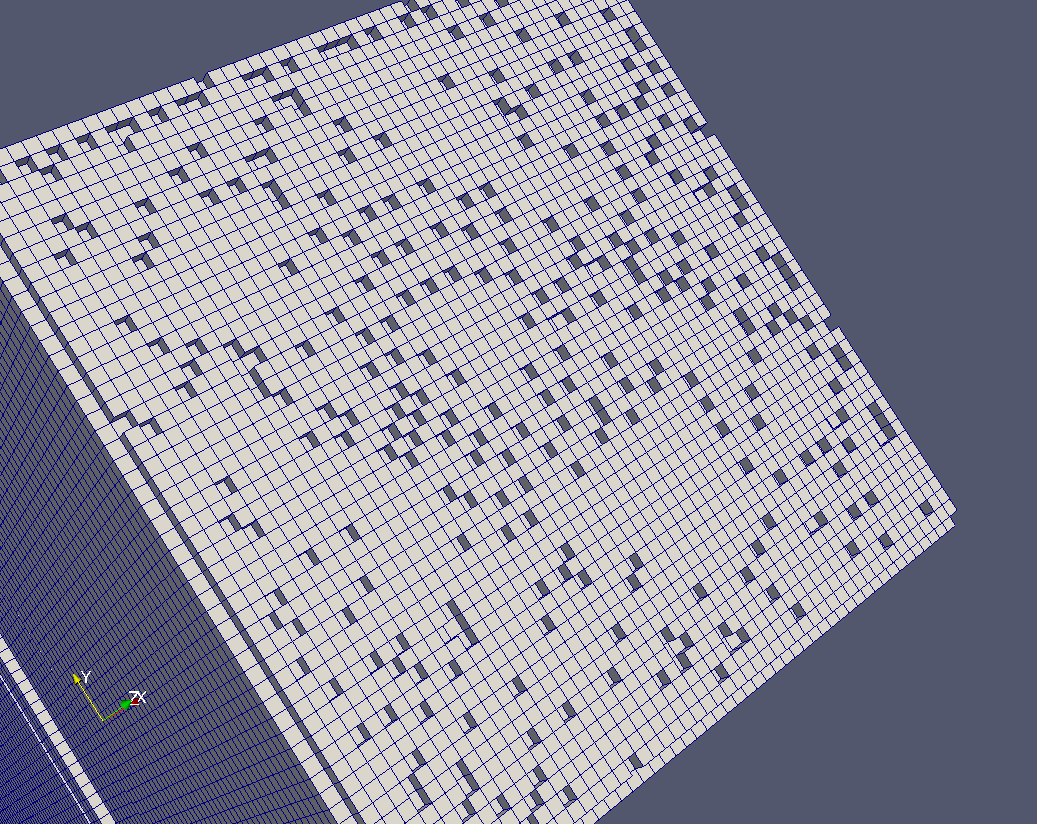
\includegraphics[width=\textwidth]{png/markers/before-refinement.png}
    \end{minipage}
    \begin{minipage}{0.49\textwidth}
        \centering
        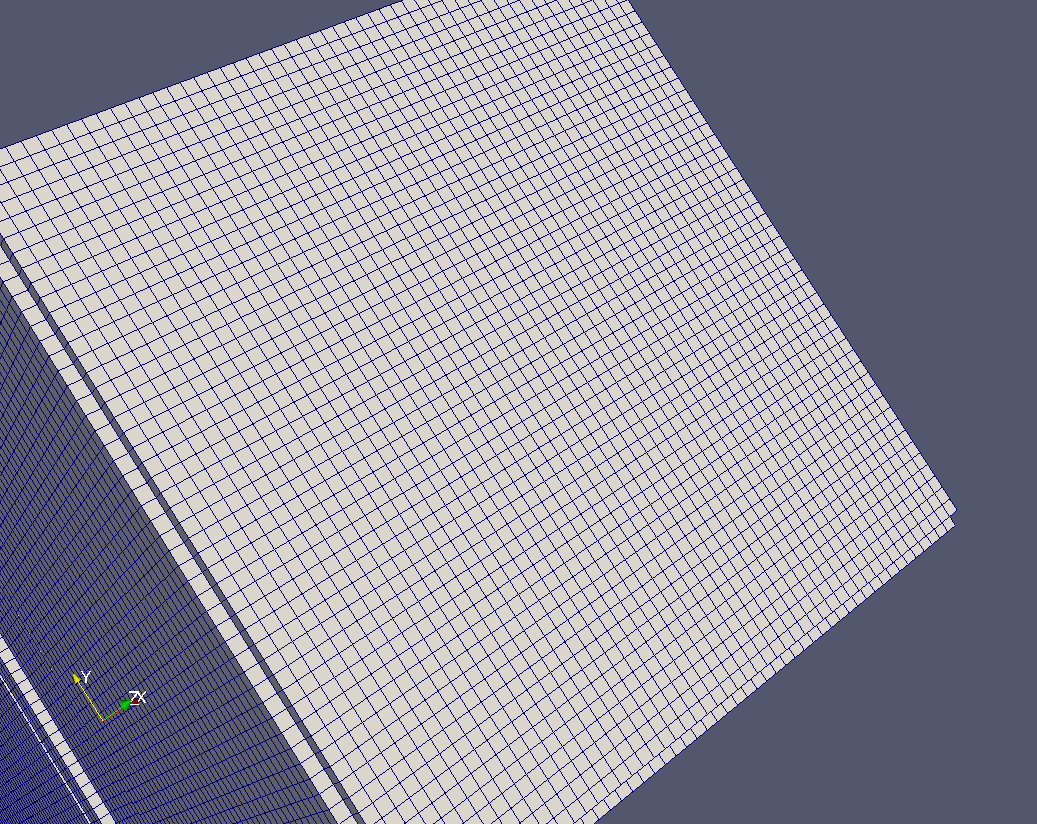
\includegraphics[width=\textwidth]{png/markers/after-refinement.png}
    \end{minipage}
}

\frame{\frametitle{Трёхмерный метод маркеров: особенности}
    Пример загруженной геометрии

    \begin{center}
        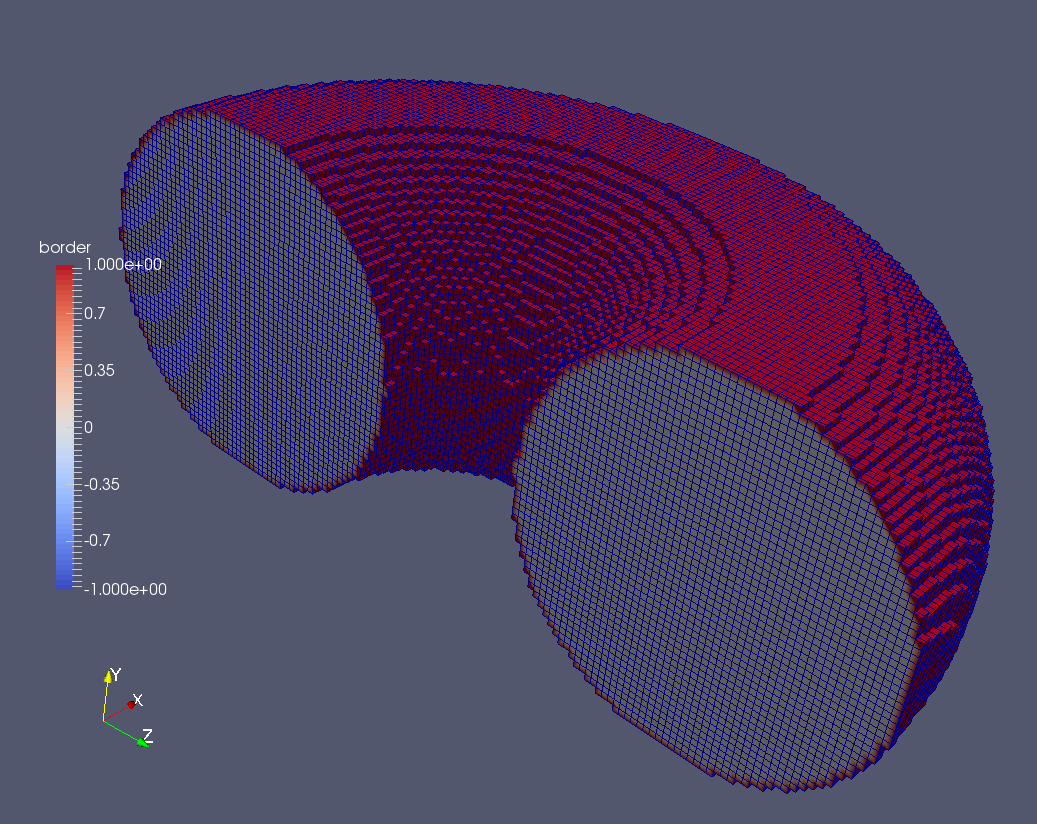
\includegraphics[width=0.7\textwidth]{png/markers/torus.png}
    \end{center}
}

\frame{\frametitle{Трёхмерный метод маркеров: особенности}
    Пример загруженной геометрии

    \begin{center}
        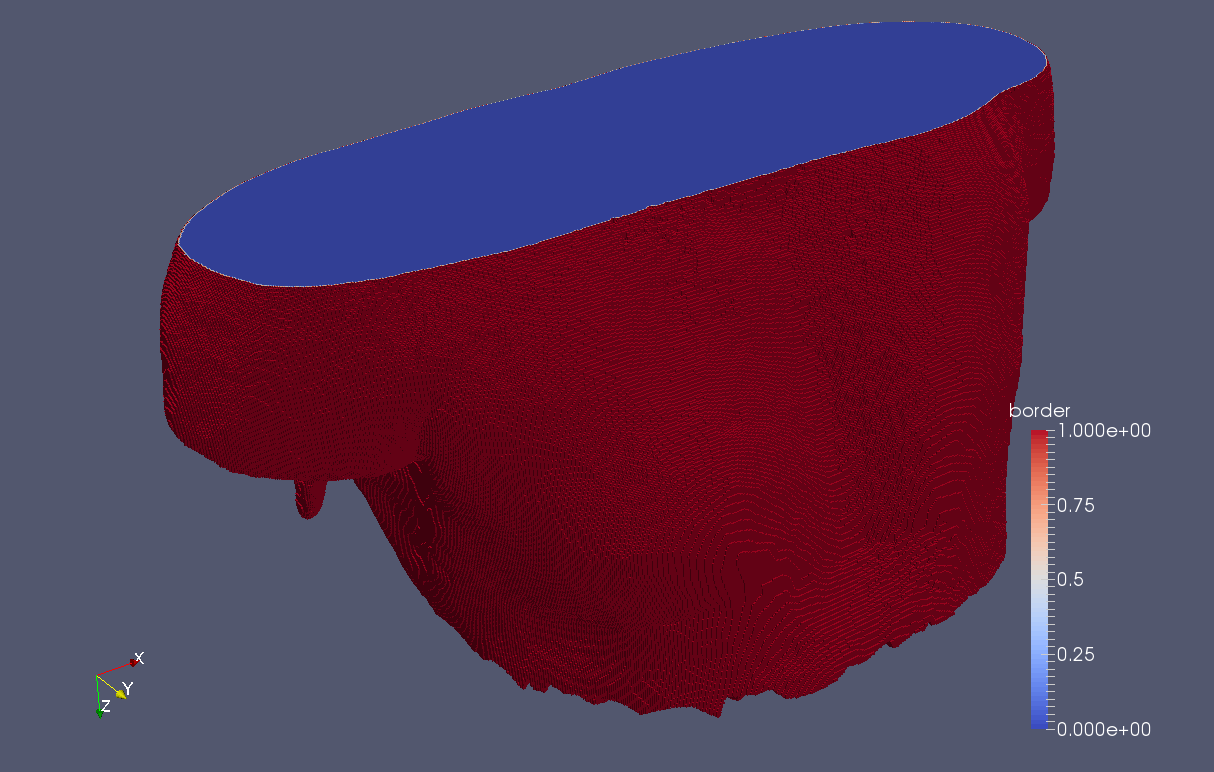
\includegraphics[width=0.8\textwidth]{png/markers/body.png}
    \end{center}
}

\frame{\frametitle{Трёхмерный метод маркеров: особенности}
    Вычисление нормалей \newline \newline
    \begin{minipage}{0.43\textwidth}
        \centering
        \tikzset{every picture/.style={scale=0.4}}\subfile{tikz/markers_cube_normals}
    \end{minipage}
    \begin{minipage}{0.52\textwidth}
        \centering
        \tikzset{every picture/.style={scale=0.4}}\subfile{tikz/markers_plane_normals}
    \end{minipage}
}

\frame{\frametitle{Трёхмерный метод маркеров: особенности}
    Экстраполяция значений \newline \newline
    \begin{minipage}{0.45\textwidth}
        \centering
        \tikzset{every picture/.style={scale=0.4}}\subfile{tikz/markers_border_interpolation_before}
    \end{minipage}
    \begin{minipage}{0.45\textwidth}
        \centering
        \tikzset{every picture/.style={scale=0.4}}\subfile{tikz/markers_border_interpolation_after}
    \end{minipage}
}

\section{Прозрачная броня: влияние адгезионной прочности}

\frame{\frametitle{Прозрачная броня: влияние адгезионной прочности}
    \begin{center}
        \begin{minipage}[h]{0.25\textwidth}
            \begin{figure}
                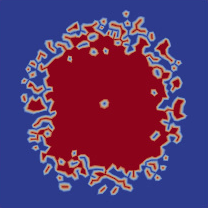
\includegraphics[width=\textwidth]{png/armor/delamination-50.png}
                \tiny
                \caption{50 МПа}
            \end{figure}
        \end{minipage}
        \begin{minipage}[h]{0.25\textwidth}
            \begin{figure}
                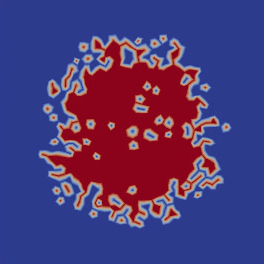
\includegraphics[width=\textwidth]{png/armor/delamination-100.png}
                \tiny
                \caption{100 МПа}
            \end{figure}
        \end{minipage}
    \end{center}
    \begin{center}
        \begin{minipage}[h]{0.25\textwidth}
            \begin{figure}
                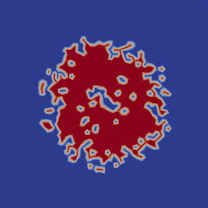
\includegraphics[width=\textwidth]{png/armor/delamination-150.png}
                \tiny
                \caption{150 МПа}
            \end{figure}
        \end{minipage}
        \begin{minipage}[h]{0.25\textwidth}
            \begin{figure}
                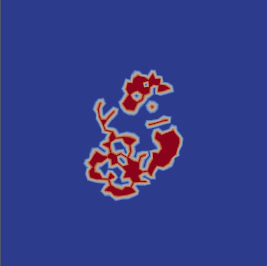
\includegraphics[width=\textwidth]{png/armor/delamination-200.png}
                \tiny
                \caption{200 МПа}
            \end{figure}
        \end{minipage}
    \end{center}
}

\section{Сравнение критериев разрушения}

\frame{\frametitle{Объёмное разрушение в~композиционном материале}
    Критерий Друкера-Прагера \newline
    \newline
    \newline
    \begin{tabular}{l|l}
        Различие пределов на~сжатие и растяжение & \Good{Да} \\
        Различие механизмов разрушения & \Bad{Нет} \\
        Мера разрушения & Скалярная \\
        Целевой материал & Субпакет \\
        Учёт наличия матрицы и воловон &  Нет \\
        Внутренние параметров модели & \Good{Нет}
    \end{tabular}
}

\frame{\frametitle{Объёмное разрушение в~композиционном материале}
    Критерий Хашина \newline
    \newline
    \newline
    \begin{tabular}{l|l}
        Различие пределов на~сжатие и растяжение & \Good{Да} \\
        Различие механизмов разрушения & \Good{Да} \\
        Мера разрушения & Скалярная \\
        Целевой материал & \Good{Монослой} \\
        Учёт наличия матрицы и воловон &  \Good{Да} \\
        Внутренние параметров модели & \Good{Нет}
    \end{tabular}
}

\frame{\frametitle{Объёмное разрушение в~композиционном материале}
    Критерий Пака \newline
    \newline
    \newline
    \begin{tabular}{l|l}
        Различие пределов на~сжатие и растяжение & \Good{Да} \\
        Различие механизмов разрушения & \Good{Да} \\
        Мера разрушения & \Good{Векторная} \\
        Целевой материал & \Good{Монослой} \\
        Учёт наличия матрицы и воловон &  \Good{Да} \\
        Внутренние параметров модели & \Bad{4}
    \end{tabular}
}

\frame{\frametitle{Объёмное разрушение в~композиционном материале}
    Критерий Цая-Хилла \newline
    \newline
    \newline
    \begin{tabular}{l|l}
        Различие пределов на~сжатие и растяжение & \Bad{Нет} \\
        Различие механизмов разрушения & \Bad{Нет} \\
        Мера разрушения & Скалярная \\
        Целевой материал & Субпакет \\
        Учёт наличия матрицы и воловон &  Нет \\
        Внутренние параметров модели & \Good{Нет}
    \end{tabular}
}

\frame{\frametitle{Объёмное разрушение в~композиционном материале}
    Критерий Цая-Ву \newline
    \newline
    \newline
    \begin{tabular}{l|l}
        Различие пределов на~сжатие и растяжение & \Good{Да} \\
        Различие механизмов разрушения & \Bad{Нет} \\
        Мера разрушения & Скалярная \\
        Целевой материал & Субпакет \\
        Учёт наличия матрицы и воловон &  Нет \\
        Внутренние параметров модели & \Good{Нет}
    \end{tabular}
}

\end{document}
